\documentclass[12pt, twoside]{article}
%\documentclass[12pt, twoside]{article}
\usepackage[letterpaper, margin=1in, headsep=0.2in]{geometry}
\setlength{\headheight}{0.6in}
%\usepackage[english]{babel}
\usepackage[utf8]{inputenc}
\usepackage{microtype}
\usepackage{amsmath}
\usepackage{amssymb}
%\usepackage{amsfonts}
\usepackage[nomessages]{fp} %\FPeval{\var-name}{2*sin(pi/6)}
\usepackage{siunitx} %units in math. eg 20\milli\meter
\usepackage{yhmath} % for arcs, overparenth command
\usepackage{tikz} %graphics
\usetikzlibrary{quotes, angles, arrows, arrows.meta}
\usepackage{pgfplots}
\usepgfplotslibrary{fillbetween}
\pgfplotsset{compat=1.16}
\usepackage{graphicx} %consider setting \graphicspath{{images/}}
\usepackage{parskip} %no paragraph indent
\usepackage{enumitem}
\usepackage{multicol}
\usepackage{venndiagram}

\usepackage{fancyhdr}
\pagestyle{fancy}
\fancyhf{}
\renewcommand{\headrulewidth}{0pt} % disable the underline of the header
\raggedbottom
\hfuzz=2mm %suppresses overfull box warnings

\usepackage{hyperref}

\fancyhead[LE]{\thepage}
\fancyhead[RO]{Markscheme}
\fancyhead[LO]{La Scuola d'Italia / Dr.\ Huson / IB Math 12 \\* 11 November 2026}

\begin{document}
\subsubsection*{3.5 Pre-Quiz: Trigonometry Review --- Markscheme}

\begin{enumerate}[itemsep=0.1cm]

%--- Problem 1: Double-angle identities: cos theta = 1/4 in quadrant IV, find sin theta, sin 2theta, cos 2theta exactly; show sin 2x/(1 + cos 2x) = tan x; hence tan theta [11 marks] ---
\item[1.] [Maximum mark: 11]

$\cos\theta = \dfrac{1}{4}$, \quad $\dfrac{3\pi}{2} < \theta < 2\pi$ (fourth
quadrant).

\textbf{(a)} $\sin^{2}\theta = 1 - \left(\dfrac{1}{4}\right)^{2}
= \dfrac{15}{16}$ \hfill \textbf{M1}

$\sin\theta = \pm\dfrac{\sqrt{15}}{4}$ \hfill \textbf{A1}

$\sin\theta = -\dfrac{\sqrt{15}}{4}$, since $\theta$ is in the fourth
quadrant \hfill \textbf{A1}

\emph{Accept a right-triangle method (sides $1$, $\sqrt{15}$, $4$) for the
M1A1. The final A1 is for the negative sign. Wrong method: the GDC route
$\sin\left(\arccos\frac{1}{4}\right) = +\frac{\sqrt{15}}{4}$ gives the
first-quadrant angle, earning M1A1A0. Decimals ($-0.968$) earn the final
A0.}

\textbf{(b)} $\sin 2\theta = 2 \times \left(-\dfrac{\sqrt{15}}{4}\right)
\times \dfrac{1}{4} = -\dfrac{\sqrt{15}}{8}$ \hfill \textbf{M1A1}

\emph{FT from (a): $+\frac{\sqrt{15}}{4}$ in (a) gives $+\frac{\sqrt{15}}{8}$,
M1A1 FT. Wrong method: $\sin 2\theta = 2\sin\theta = -\frac{\sqrt{15}}{2}$
earns M0A0.}

\textbf{(c)} $\cos 2\theta = 2 \times \left(\dfrac{1}{4}\right)^{2} - 1
= -\dfrac{7}{8}$ \hfill \textbf{M1A1}

\emph{Accept any of the three forms, e.g.\ $\frac{1}{16} - \frac{15}{16}$
or $1 - 2 \times \frac{15}{16}$. Wrong method: $\cos 2\theta = 2\cos\theta
= \frac{1}{2}$ earns M0A0. A value outside $[-1, 1]$ signals an error.}

\textbf{(d)} $\dfrac{\sin 2x}{1 + \cos 2x}
= \dfrac{2\sin x\cos x}{1 + 2\cos^{2}x - 1}$ \hfill \textbf{M1}

$= \dfrac{2\sin x\cos x}{2\cos^{2}x}$ \hfill \textbf{A1}

$= \dfrac{\sin x}{\cos x}$ \hfill \textbf{A1}

$= \tan x$ \hfill \textbf{AG}

\emph{M1 for substituting both double-angle identities. The form
$\cos 2x = 2\cos^{2}x - 1$ is the efficient choice; $\cos^{2}x - \sin^{2}x$
also works, with $1 - \sin^{2}x = \cos^{2}x$. Wrong method: checking one
value, e.g.\ $x = \frac{\pi}{4}$, proves nothing and earns M0.}

\textbf{(e)} $\tan\theta = \dfrac{-\frac{\sqrt{15}}{8}}{1 - \frac{7}{8}}
= -\sqrt{15}$ \hfill \textbf{A1}

\emph{Or otherwise: $\tan\theta = \frac{\sin\theta}{\cos\theta}
= \frac{-\sqrt{15}/4}{1/4}$. FT from (b) and (c), or from (a). Inverted
ratio $-\frac{1}{\sqrt{15}}$ earns A0. $+\sqrt{15}$ earns A0 unless it
follows from the candidate's $+\frac{\sqrt{15}}{4}$ in (a).}

\newpage

%--- Problem 2: Bearings: ship sails 12 km on 070 then 9 km on 170; show angle HAB = 80 deg; HB by cosine rule; bearing of B from H via sine rule; back bearing; area [12 marks] ---
\item[2.] [Maximum mark: 12]

$HA = 12$ km on $070^\circ$, then $AB = 9$ km on $170^\circ$.

\textbf{(a)} bearing of $H$ from $A$ $= 070^\circ + 180^\circ = 250^\circ$
\hfill \textbf{M1}

$H\hat{A}B = 250^\circ - 170^\circ = 80^\circ$ \hfill \textbf{A1 AG}

\emph{Accept any correct angle argument at $A$, e.g.\ the angle between
$[AH]$ and the south line at $A$ is $70^\circ$ (alternate angles) and the
angle between $[AB]$ and the south line is $10^\circ$, so
$70^\circ + 10^\circ = 80^\circ$; or the ship turns through
$170^\circ - 70^\circ = 100^\circ$, so $H\hat{A}B = 180^\circ - 100^\circ$.}

\textbf{(b)} $HB^{2} = 12^{2} + 9^{2} - 2 \times 12 \times 9\cos 80^\circ$
\hfill \textbf{M1A1}

$HB = 13.7$ km \quad $(13.6927\ldots)$ \hfill \textbf{A1}

\emph{M1 for substituting into the cosine rule, A1 for the correct
substitution. $HB^{2} = 187.491\ldots$. Wrong methods: the angle
$100^\circ$ gives $16.2$, M1A0A0; radian mode gives $15.8$
(15.7747\ldots), M1A1A0.}

\textbf{(c)} $\dfrac{\sin A\hat{H}B}{9} = \dfrac{\sin 80^\circ}{13.6927\ldots}$
\hfill \textbf{M1}

$A\hat{H}B = 40.3^\circ$ \quad $(40.3380\ldots)$ \hfill \textbf{A1}

bearing $= 70^\circ + 40.3380\ldots^\circ$ \hfill \textbf{M1}

$= 110^\circ$ \quad $(110.338\ldots)$ \hfill \textbf{A1}

\emph{Accept $110.3^\circ$. Accept the cosine rule for $A\hat{H}B$. The
angle is opposite the shorter side $9 < 13.69$, so it is acute: no
ambiguous case. FT from (b). Wrong methods: $40.3^\circ$ given as the
bearing, M1A1M0A0; $70^\circ - 40.3^\circ = 29.7^\circ$, M1A1M0A0; the angle
at $B$, $59.7^\circ$, added to $70^\circ$ gives $130^\circ$, M0A0M1A0.}

\textbf{(d)} $110.338\ldots^\circ + 180^\circ = 290^\circ$
\quad $(290.338\ldots)$ \hfill \textbf{A1}

\emph{Accept $290.3^\circ$. FT from (c). Wrong methods, each A0:
$360^\circ - 110^\circ = 250^\circ$; $180^\circ - 110^\circ = 70^\circ$.}

\textbf{(e)} area $= \dfrac{1}{2} \times 12 \times 9\sin 80^\circ$
\hfill \textbf{M1}

$= 53.2\ \text{km}^{2}$ \quad $(53.1796\ldots)$ \hfill \textbf{A1}

\emph{Accept any two sides with their included angle, e.g.\
$\frac{1}{2} \times 12 \times 13.6927\ldots \sin 40.3380\ldots^\circ$. Wrong
method: an angle not included between the two sides, e.g.\
$\frac{1}{2} \times 12 \times 13.69\sin 80^\circ = 80.9$, earns M0A0.
Note: $\sin 100^\circ = \sin 80^\circ$, so the wrong angle from (a) gives
the correct area; (a) fixes the angle at $80^\circ$.}

\newpage

%--- Problem 3: Equations with double angles on [0, 2pi]: sin 2x = sin x (factorise, do not divide by sin x); cos 2x + 3cos x + 2 = 0 as a quadratic in cos x [11 marks] ---
\item[3.] [Maximum mark: 11]

\textbf{(a)} $2\sin x\cos x = \sin x$ \hfill \textbf{M1}

$2\sin x\cos x - \sin x = 0$

$\sin x\,(2\cos x - 1) = 0$ \hfill \textbf{M1}

$\sin x = 0$ \quad or \quad $\cos x = \dfrac{1}{2}$

$x = 0,\ \pi,\ 2\pi$ \hfill \textbf{A1}

$x = \dfrac{\pi}{3},\ \dfrac{5\pi}{3}$ \hfill \textbf{A1A1}

\emph{Second M1 for factorising (or for setting each factor to zero).
The A1 for $\sin x = 0$ needs all three values. Wrong method: dividing by
$\sin x$ loses $0$, $\pi$, $2\pi$ and earns M1M0A0A1A1. Missing the end
points $0$ or $2\pi$ earns A0 for that line. Decimals ($1.05$, $3.14$,
$5.24$) earn at most one of the three A1.}

\textbf{(b)(i)} $\cos 2x + 3\cos x + 2 = 2\cos^{2}x - 1 + 3\cos x + 2$
\hfill \textbf{M1}

$= 2\cos^{2}x + 3\cos x + 1$ \hfill \textbf{A1 AG}

\emph{M1 for choosing the form $\cos 2x = 2\cos^{2}x - 1$. The forms
$\cos^{2}x - \sin^{2}x$ or $1 - 2\sin^{2}x$ earn the M1 only when
$\sin^{2}x$ is then replaced by $1 - \cos^{2}x$.}

\textbf{(b)(ii)} $(2\cos x + 1)(\cos x + 1) = 0$ \hfill \textbf{M1}

$\cos x = -\dfrac{1}{2}$ \quad or \quad $\cos x = -1$ \hfill \textbf{A1}

$x = \dfrac{2\pi}{3},\ \dfrac{4\pi}{3}$ \hfill \textbf{A1}

$x = \pi$ \hfill \textbf{A1}

\emph{Accept the quadratic formula, or a substitution $u = \cos x$, for
the M1. Wrong method: a sign error in the factors, $\cos x = \frac{1}{2}$
or $1$, gives $x = 0, \frac{\pi}{3}, \frac{5\pi}{3}, 2\pi$: M1A0, then
A1A1 FT. Missing $x = \pi$ (a single value from $\cos x = -1$) is the
most common loss. Decimals ($2.09$, $3.14$, $4.19$) earn at most A1 of the
last two.}

\newpage

%--- Problem 4: f(x) = 6 sin x cos x + 1 on [0, pi]: show f = 3 sin 2x + 1; period; range; sketch; solve f(x) = 2.5 exactly; values of k for exactly two solutions of f(x) = k [13 marks] ---
\item[4.] [Maximum mark: 13]

$f(x) = 6\sin x\cos x + 1$, \quad $0 \le x \le \pi$.

\textbf{(a)} $6\sin x\cos x = 3 \times 2\sin x\cos x$ \hfill \textbf{M1}

$= 3\sin 2x$, so $f(x) = 3\sin 2x + 1$ \hfill \textbf{A1 AG}

\textbf{(b)} period $= \dfrac{2\pi}{2} = \pi$ \hfill \textbf{A1}

\emph{Wrong methods, each A0: $2\pi$ (the period of $\sin x$); $2$.}

\textbf{(c)} maximum $= 3 + 1 = 4$, \ minimum $= -3 + 1 = -2$, so
$-2 \le f(x) \le 4$ \hfill \textbf{A1A1}

\emph{A1 for each end point with the correct inequality. Accept $[-2, 4]$.
The end points are included: $f\left(\frac{\pi}{4}\right) = 4$ and
$f\left(\frac{3\pi}{4}\right) = -2$. Strict inequalities earn A1A0. Wrong
methods: $-3 \le f(x) \le 3$ (the $+1$ ignored) or $-5 \le f(x) \le 7$
(amplitude $6$), A0A0.}

\textbf{(d)}

\begin{minipage}[c]{0.42\linewidth}
\centering
\begin{tikzpicture}[xscale=1.3, yscale=0.42]
  \foreach \x in {0.5,1,...,4} \draw[gray!40] (\x,-3) -- (\x,5);
  \foreach \y in {-3,...,5} \draw[gray!40] (0,\y) -- (4.2,\y);
  \draw[->] (0,0) -- (4.35,0) node[right] {$x$};
  \draw[->] (0,-3.2) -- (0,5.4) node[above] {$y$};
  \foreach \x/\l in {1/{\frac{\pi}{4}},2/{\frac{\pi}{2}},3/{\frac{3\pi}{4}},4/{\pi}}
    \node[below, fill=white, inner sep=1pt] at (\x,-0.12) {\small $\displaystyle\l$};
  \foreach \y in {-2,2,4}
    \node[left] at (0,\y) {\footnotesize $\y$};
  % solution curve: y = 3 sin 2x + 1, with x in units of pi/4, so 2x = (pi/2) u
  \draw[very thick, domain=0:4, samples=120, smooth]
    plot (\x, {3*sin(90*\x) + 1});
  \foreach \p in {(0,1),(1,4),(2,1),(3,-2),(4,1)} \fill \p circle (1.5pt);
  \node[above] at (1,4) {\footnotesize $\left(\frac{\pi}{4}, 4\right)$};
  \node[below right] at (3,-2) {\footnotesize $\left(\frac{3\pi}{4}, -2\right)$};
\end{tikzpicture}
\end{minipage}
\hfill
\begin{minipage}[c]{0.54\linewidth}
shape: one complete sine wave \hfill \textbf{A1}

\smallskip
maximum $\left(\tfrac{\pi}{4}, 4\right)$, minimum
$\left(\tfrac{3\pi}{4}, -2\right)$ \hfill \textbf{A1}

\smallskip
$y = 1$ at $x = 0, \tfrac{\pi}{2}, \pi$; domain $[0, \pi]$ \hfill \textbf{A1}
\end{minipage}

\emph{The $x$-intercepts are $1.74$ (1.74071\ldots) and $2.97$
(2.97169\ldots); they need not be labelled. Wrong method: two cycles
(period $\frac{\pi}{2}$) or half a cycle (period $2\pi$) earns A0 for the
shape. FT from (b) and (c).}

\textbf{(e)} $3\sin 2x + 1 = 2.5$, \ so \ $\sin 2x = \dfrac{1}{2}$ \hfill \textbf{M1}

$2x = \dfrac{\pi}{6},\ \dfrac{5\pi}{6}$ \quad (for $0 \le 2x \le 2\pi$)

$x = \dfrac{\pi}{12},\ \dfrac{5\pi}{12}$ \hfill \textbf{A1A1}

\emph{Wrong methods: $x = \frac{\pi}{6}, \frac{5\pi}{6}$ (not halved)
earns M1A0A0; $\frac{\pi}{12}$ only earns M1A1A0; $\sin 2x = \frac{2.5}{3}$
(the $+1$ ignored) earns M0. Extra values outside $0 \le x \le \pi$, e.g.\
$\frac{13\pi}{12}$, earn the final A0. Decimals ($0.262$, $1.31$) earn A1A0
at most.}

\textbf{(f)} $-2 < k < 1$ \quad or \quad $1 < k < 4$ \hfill \textbf{A1A1}

\emph{Accept $-2 < k < 4$, $k \neq 1$. From the sketch: $k = 1$ gives three
solutions ($0$, $\frac{\pi}{2}$, $\pi$), and $k = 4$ or $k = -2$ gives one.
Wrong methods: $-2 < k < 4$ with $k = 1$ not excluded earns A1A0;
including $k = -2$ or $k = 4$ earns A0 for that interval.}

\end{enumerate}
\end{document}
